%%
%% This is file `squelette-rr.tex',
%% generated with the docstrip utility.
%%
%% The original source files were:
%%
%% RR.dtx  (with options: `sample')
%% ********************************************************************
%% Copyright (C) 1997-1999 2004 2006-2011 INRIA/APICS/MARELLE by Jose' Grimm
%% This file may be distributed and/or modified under the
%% conditions of the LaTeX Project Public License, either version 1.3
%% of this license or (at your option) any later version.
%% The latest version of this license is in
%%    http://www.latex-project.org/lppl.txt
%% and version 1.3 or later is part of all distributions of LaTeX
%% version 2003/12/01 or later.
%% An archive of the software can be found at
%%    ftp://ftp-sop.inria.fr/marelle/RR-INRIA

\documentclass[twoside]{article}
\usepackage[a4paper]{geometry}
\usepackage[utf8]{inputenc} % use UTF-8 input encoding
\usepackage[T1]{fontenc} % ou \usepackage[OT1]{fontenc}
\usepackage{RR}
\usepackage{hyperref}
\usepackage{bookmark} % improve outline handling, avoids rerun warnings
\usepackage[norule]{footmisc} % pour supprimer le filet des notes
\usepackage{tikz}
\usetikzlibrary{shapes,arrows,positioning}

%%\usepackage[frenchb]{babel} % optionnel
\RRNo{XXXX}
%% \RTNo{0703}
%%
%% date de publication du rapport
\RRdate{MONTH YEAR}
%%
%% Cas d'une version deux
%% \RRversion{2}
%% date de publication de la version 2
%% \RRdater{November 2008}
%%\RRversion{2\thanks{la note explicative}}
\RRdater{MONTH YEAR} % date de revision du rapport
\RRauthor{% les auteurs
 % Premier auteur, avec une note
Alexandre Lou-Poueyou\thanks{Computer Science Master's Degree Student at University of Bordeaux - Intern at TADaaM team}%
 % \and entre chaque auteur s'il y en a plusieurs
  \and
Francieli Boito\thanks{Associate Professor at University of Bordeaux \& permanent researcher at TADaaM team}%
 % r\'ef\'erence \`a la note partag\'ee
 % liste longue pour tests de mise en page
\and Meline Trochon\thanks{PhD stutent at TADaaM team} \and Luan Teylo \thanks{Permanent researcher at TADaaM team}}
%% Ceci apparait sur chaque page paire.
\authorhead{Alexandre \& Francieli \& others}
%% titre francais long
\RRtitle{Exemple de document\\
 utilisant le style\\rapport de recherche\\Inria}
%% English title
\RRetitle{Improving I/O Performances of HPC Application Gysela}
%%
\titlehead{Improving I/O performances of HPC Application Gysela}
%%
%\RRnote{This is a note}
%\RRnote{This is a second note}
%%
\RRresume{Ce document montre comment utiliser le style RR.sty.
Pour en savoir plus, consulter le fichier RR.dvi ou RR.pdf.
D\'efinissez toujours les commandes avant utilisation.
}
\RRabstract{
In modern High-Performance Computing (HPC) systems, Input/Output (I/O) performance 
is a major bottleneck for large-scale scientific simulations. As computational power 
and data volumes scale rapidly, optimizing I/O workflows becomes critical to efficiently 
leverage supercomputing resources. Scientific applications heavily rely on Parallel File 
Systems (PFS) to access vast datasets concurrently. However, achieved performance is highly 
sensitive to PFS configurations, high-level I/O strategies, and application-specific access patterns. 
Understanding and tuning the interactions between these layers is crucial for maximizing global simulation throughput.\\
This work focuses on optimizing the checkpointing performance of Gysela, a 5D gyrokinetic simulation code 
developed by the CEA for nuclear fusion research. Gysela generates massive datasets and relies on periodic 
checkpointing for fault tolerance and job restartability. Using gys\_io, a lightweight mini-app replicating 
Gysela’s parallel I/O patterns, we systematically evaluate and compare different parallel I/O strategies—namely 
Single Shared File (SSF), Subfiling, and File Per Process (FPP)—alongside key PFS configuration parameters. 
Our experiments, conducted on diverses clusters, analyze the performance trade-offs of these strategies 
and parameters under various scaling conditions. The results identify optimal parallel configurations, 
clarify the impact of PFS striping on each I/O strategy, and provide actionable optimization recommendations 
to significantly reduce checkpointing overhead in future Gysela production runs.
}
\RRkeyword{HPC, Parallel I/O, Performances Tuning, Parallel File Systems}
%%
%% \RRprojet{Apics}  % cas d'un seul projet
\RRprojets{TADaaM}
%%
%% \URLorraine % pour ceux qui sont \`a l'est
%% \URRennes  % pour ceux qui sont \`a l'ouest
%% \URRhoneAlpes % pour ceux qui sont dans les montagnes
%% \URRocq % pour ceux qui sont au centre de la France
%% \URFuturs % pour ceux qui sont dans le virtuel
%% \URSophia % pour ceux qui sont au Sud.
%%
%% \RCBordeaux % Centre Inria de l'Université de Bordeaux
%% \RCGrenoble % Centre Inria de l'Université de Grenoble Alpes
%% \RCLille % Centre Inria de l'Université de Lille
%% \RCLyon % Centre Inria de Lyon
%% \RCNancy % Centre Inria de l'Université de Lorraine
%% \RCParis % Centre Inria de Paris
%% \RCRennes % Centre Inria de l'Université de Rennes 
%% \RCSaclay % Centre Inria de Saclay
%% \RCSophia % Centre Inria d'Université Côte d'Azur


\RCBordeaux

%%
\begin{document}
%%
%\makeRR   % cas d'un rapport de recherche
\makeRT % cas d'un rapport technique.
%% a partir d'ici, chacun fait comme il le souhaite
\tableofcontents \newpage

\section{Introduction}
\label{sec:intro}

In modern High-Performance Computing (HPC) systems, Input/Output (I/O) performance has become nearly critical as computational
power itself. As supercomputer advance toward exascale capabilities, computational throughput has increased exponentially, yet
storage bandwidth has lagged behind. This growing imbalance creates a fundamental bottleneck: while modern processors achieve teraflop-
scale performance, parallel file systems typically deliver only tens to hundreds of gigabytes per second in aggregate bandwidth.
Figure \ref{fig:io_per_flop} quantifies this imbalance using data from major supercomputers from 2000 to 2025. The I/O bandwidth 
per unit of compute (measured in GBps per PetaFlop) has declined from $\sim$300 GBps/PF on ASCI Red (2000) to only $\sim$6 GBps/PF 
on Frontier (2023) a 50-fold degradation. This trend accelerated sharply after 2015, demonstrating that I/O has become the dominant 
bottleneck for modern exascale systems.

\begin{figure}[h]
  \centering
  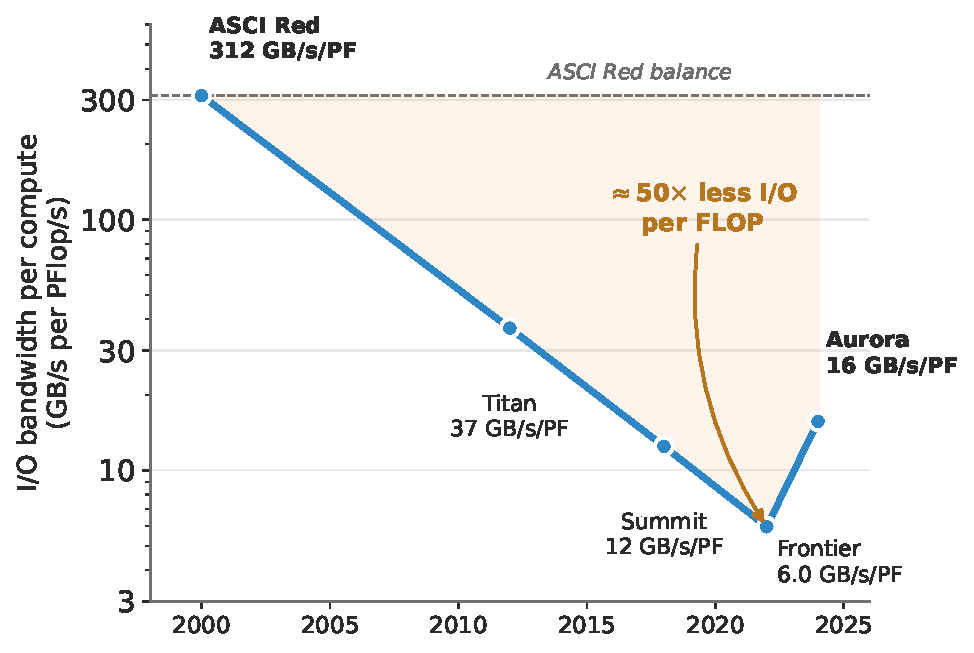
\includegraphics[width=0.5\textwidth]{figures/io_per_flop.pdf}
  \caption{Compute-to-I/O performance gap in top 500 supercomputers (2000--2025).\\
  The ratio of computational throughput to storage bandwidth has grown by an order of indicating that I/O is increasingly the limiting factor.}
  \label{fig:io_per_flop}
\end{figure}

Large-scale scientific simulations generate massive data volumes requiring efficient I/O management. On parallel file systems, thousands of processes 
must coordinate concurrent access to shared storage while contending for limited bandwidth.
Gysela is a 5D gyrokinetic simulation code developed by the CEA (Commissariat à l'\'energie Atomique) for nuclear fusion research. It models plasma turbulence 
in tokamaks by solving the Vlasov equation in a five-dimensional phase space: three spatial coordinates (minor radius and two toroidal angles) and two velocity-space 
coordinates (parallel velocity and magnetic moment). Understanding and controlling the turbulence that degrades plasma confinement is crucial for the success of 
next-generation fusion reactors like ITER.
Production Gysela simulations run thousands of processes and generate massive checkpoint datasets. Due to the long execution times (ranging
from days to weeks on large allocations) and the constant risk of hardware failures or job time limits on production systems, Gysela relies on
periodic checkpointing saving the complete simulation state at regular intervals to enable clean restarts without recomputing from the beginning.
The checkpointing writing process is synchronous: All MPI ranks pause computation and collectively write their portion of the 5D state to persistent storage.
During this phase, expensive supercomputer resources sit idle, wasting valuable compute hours. In production environments, checkpoints write time suffers from
significant variability-sometimes exceeding the mean by a factor of 3 or more-due to PFS contention with other jobs and variable network behavior. This unpredictability
difficult to accurately predict job completion times and optimize checkpoint frequency.
Optimizing checkpoint I/O requires simultaneous attention to two distinct challenges: tunin parallel file system configuration parameters (e.g., stripe count, stripe size and OST allocation) detailled in section \ref{sec:background}
and selecting an appropriate I/O strategy (how application data is organized and written to the PFS).
To facilitate rapid, reproducible experimentation, we use {\tt gys\_io}, a lightweight mini-application that replicates Gysela's 5D checkpoint pattern without the computational burden. 
This mini-app enables benchmarking to complete in seconds per configuration rather than hours, allowing systematic parameter sweeps across hundreds of experiments. Importantly, {\tt gys\_io}
accepts the same configuration files as Gysela, ensuring that benchmark results directly inform production deployments. Optimizing checkpoint I/O requires tuning both parallel file system configuration parameters 
and selecting an appropriate I/O strategy. This work evaluates three complementary approaches and identifies the most effective configurations for Gysela.


\section{Context} % Part of the report where i talk about Inria, TADaaM, NumPex & Exa-Dost
\label{sec:context}

This work is conducted at Inria, the French National Institute for Research in Digital Science and Technology. Inria is internationally recognized for its major contributions to high-performance computing, artificial intelligence,
and computer networks. With ten research centers across France and over 3,500 researchers, engineers, and administrative staff, Inria leads fundamental and applied research in computer science and mathematics with a focus on societal impact.

This intership is part of the TADaaM team (Topology-Aware system-scale Data management for high-performance computing) at the Inria Bordeaux research center. TADaaM is dedicated to designing a comprehensive service layer for HPC systems, enabling
applications to express their resource requirements and allowing the system to dynamically optimize execution at scale. The team's work bridges application needs and system capabilities,
ensuring efficient utilization of large-scale computing resources.

This research is part of the NumPex project, a European HPC research initiative dedicated to preparing Europe's scientific computing ecosystem for the exascale era. NumPex brings together leading research institutions, HPC centers, and industry
paterns to develop and validate technologies for extreme-scale simulation and data processing. This work contributes to Exadost, a NumPex work package focused on optimizing I/O performance and data management strategies for exascale applications.

The Gysela application studied in this work is developed by the CEA (Commissariat à l'énergie Atomique et aux énergies alternatives), France's atomic and alternative energies commission. Gysela is used by CEA researchers to study plasma turbulence in
fusion reactors, making I/O optimization critical for advacing fusion energy research on future exascale systems.


section \ref{sec:intro} on page \pageref{sec:intro}.





\section{Background}
\label{sec:background}

\subsection{Parralel File System}

\begin{itemize}
  \item Difference between File System and Parallel File System is striping concept
  \item Multiple PFS exist : BeegFS, Lustre, ...
  
  \item OST stand for Object Storage Target
  \item OST is a physical and logical unit measure represented by hard disk or group of disk
  \item Allows data to be partitioned across multiple storage systems

  \item Striping is a data distribution technique
  \item Cut datas into multiple chunk called stripe
  \label{ref:stripe_size}
  \item Those chunks are written on OSTs
  
  \item Main objective of PFS is to improve bandwidth usage
\end{itemize}

\subsection{Write Strategy}

We implement three distinct I/O strategies Single Shared File (SSF), Subfiling and File Per Process (FPP) using PDI (Parallel Data Interface), a middleware layer developped by {\tt Maison de la simulation} team that
decouple I/O strategy from application code. Each strategy is selected by modifying a YAML configuration file; no code recompilation is required. This flexibility allows rapid evaluation of strategies
and enables production systems to adapt I/O policies without code maintenance overhead.


\subsubsection{Single Shared File}

\begin{itemize}
  \item Every processes write on a same file
  \item Two-Phase I/O
  \item First Data aggregation and then send to PFS
\end{itemize}

\begin{figure}[h]
  \centering
  \begin{minipage}{0.7\textwidth}
    \centering
    \input{figures/ssf_background.tex}
  \end{minipage}
  \caption{Illustration of the Single Shared File (SSF) strategy.}
  \label{fig:ssf_background}
\end{figure}

\subsubsection{Subfiling}

\begin{itemize}
  \item Processes's data are aggregated into a smaller number of files called subfiles
  \item Each subfile is written to the PFS by a single process (IO Concentrator)
  \item Number of subfiles is a tunable parameter that can be adjusted to optimize performance based on each applications.
  \item Writing phase of subfiles is done by chunks of data called stripes size \ref{ref:stripe_size} that are written in parallel on the PFS
  \item Subfiling strategy aims to reduce contention on the PFS by decreasing the number of concurrence write operations.
\end{itemize}

\begin{figure}[h]
  \centering
  \begin{minipage}{0.7\textwidth}
    \centering
    \input{figures/subfiling_background.tex}
  \end{minipage}
  \caption{Illustration of the Subfiling strategy.}
  \label{fig:subfiling_background}
\end{figure}

\subsubsection{File Per Process}

\begin{itemize}
  \item Each process writes its own file on the PFS
  \item This strategy is simple to implement and does not require any data aggregation or coordination between
  \item However, it can lead to a large number of small files, which may cause performance issues on some PFS due to metadata overhead and file system limitations.
\end{itemize}

\begin{figure}[h]
  \centering
  \begin{minipage}{0.7\textwidth}
    \centering
    \input{figures/fpp_background.tex}
  \end{minipage}
  \caption{Illustration of the File Per Process (FPP) strategy.}
  \label{fig:fpp_background}
\end{figure}

\subsection{Software Stacks \& Tools}

\subsubsection{Gysela Mini App IO}

\begin{itemize}
  \item Gysela is 
\end{itemize}

\subsubsection{PDI}

\subsubsection{IOPS}

\subsubsection{TOTO}

\section{Experimental Set-up}

\newpage
% Bibliography style (none used in this template, but ensures \bibstyle is set)
\bibliographystyle{plain}

\end{document}
\endinput
%%
%% End of file `squelette-rr.tex'.
